\chapter{The visualization techniques}
\label{chap:visualization}

In this chapter, we will survey current existing works on the
visualization of the information diffusion. Generally, most of
the work about the visualization is how to visualize the social
network. Also, there are some papers talking about spreading of the
disease which is similiar to information diffusion. At the last of the
chapter, we will summarize some visualization techniques that could be
used in information diffusion.

\section{Social network visualization}

There are already some surveys about visualizing the social
networks~\cite{freeman2000visualizing}
~\cite{correa2011visualizing}. 
In \cite{correa2011visualizing}, Correa gave a taxonomy of
visualization of the social networks. He classified the
visualization of the social networks into four main groups: structural
visualization, semantic visualization, temporal visualization, and
statistical visualization. Now we will explain these four groups in
detail:

\textit{Structural visualization}:

\begin{figure}[!htb]
  \centering
  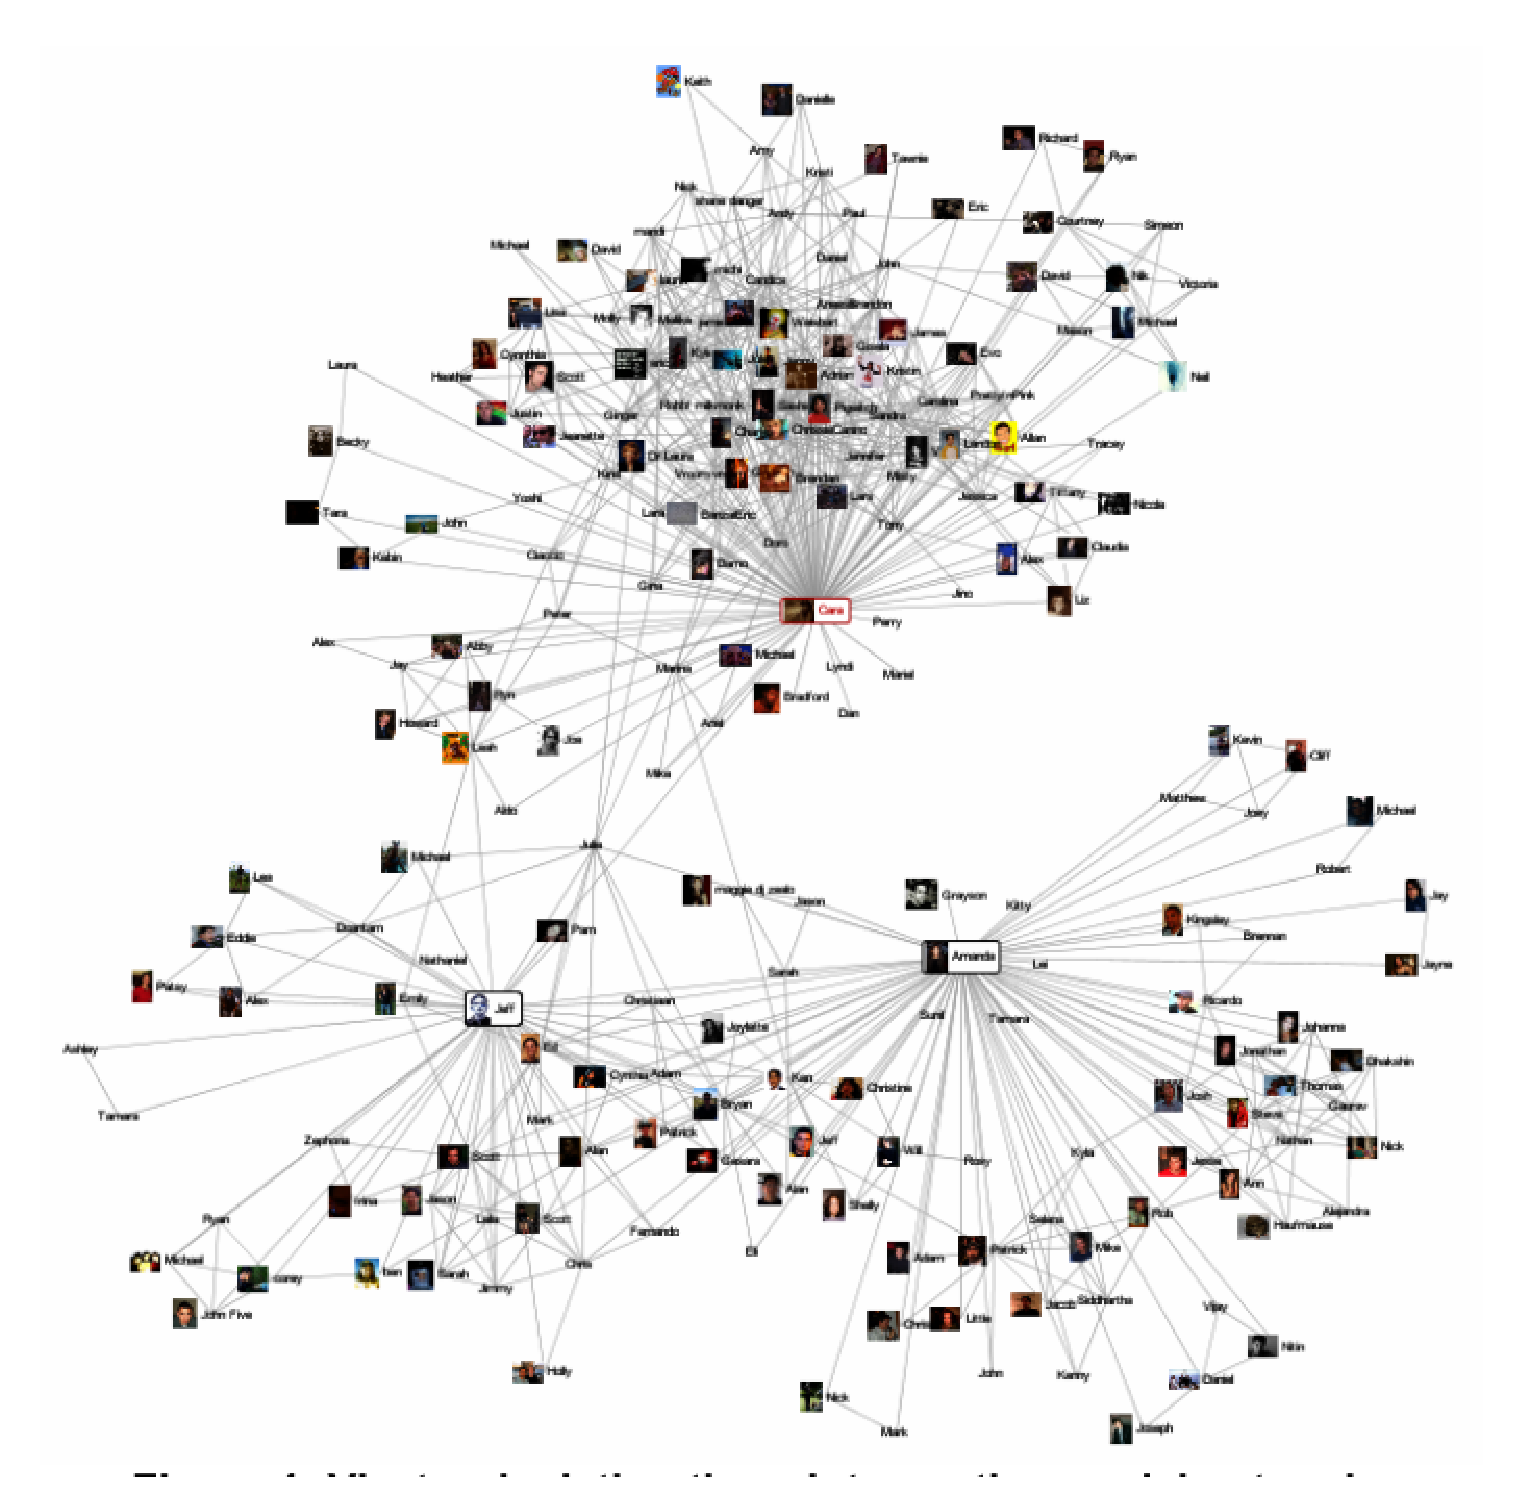
\includegraphics[width = 300px]{figures/nodelink.eps}
  \caption{An example of node-link method for the structure
    visualization ~\cite{heer2005vizster}}
  \label{fig:nodelink}
\end{figure}

\begin{figure}[!htb]
  \centering
  \includegraphics[width = 500px]{figures/edgebundle.eps}
  \caption{Figure (a) shows the raw edges of the graph, and Figure (b) shows the result after the edge bundling.}
  \label{fig:edgebundle}
\end{figure}


The structural visualization focuses on how to visualize topology of a
graph extracted from a social network. Basically, there are two
different methods: the node-link method and the matrix method.

The node-link method is a very straightforward method that visualizes the
topology of the graph. As the real social network is ususaly very
huge, and it grows in complexity and size, a serious challenge for us
to visualizing it is how to find a good layout algorithm. Currently,
there are some techniques on graph visualization, which can be very
helpful for us to solve this problem. For example, in~\cite{holten2006hierarchical},
Holten proposed the hierarchical edge bundling algorithm to reduce the visual clutter (See Figure~\ref{fig:edgebundle}).

The matrix-oriented method is to represent a social network via an
explicit display of its adjacency or incidence matrix. In this
visualization, each link is represented as a grid location with
cartesian coordinates corresponding to the nodes in the
network. Color and opacity are often used to represent important
structural or semantic quantities. Consequently, a visual
representation of the adjacency matrix is much more compact than a
node-link method and overlap-free, since each link is represented
without overlap.

These two methods are indeed complementary. Thus, combining them
together is a good choice, which we call the hybrid method. The work done by Henry et al. is a very
typical example of the hybrid method~\cite{henry2007nodetrix}. They
proposed a new visualization called NodeTrix, using the node-link
method to visualize the overall structure of the network and using the
adjacency matrices to show the commnunities(See Figure~\ref{fig:nodetrix}).
Besides, the visualizations ~\cite{shen2007path} and
~\cite{muelder2008rapid} are also the hybrid methods.

\begin{figure}[!htb]
  \centering
  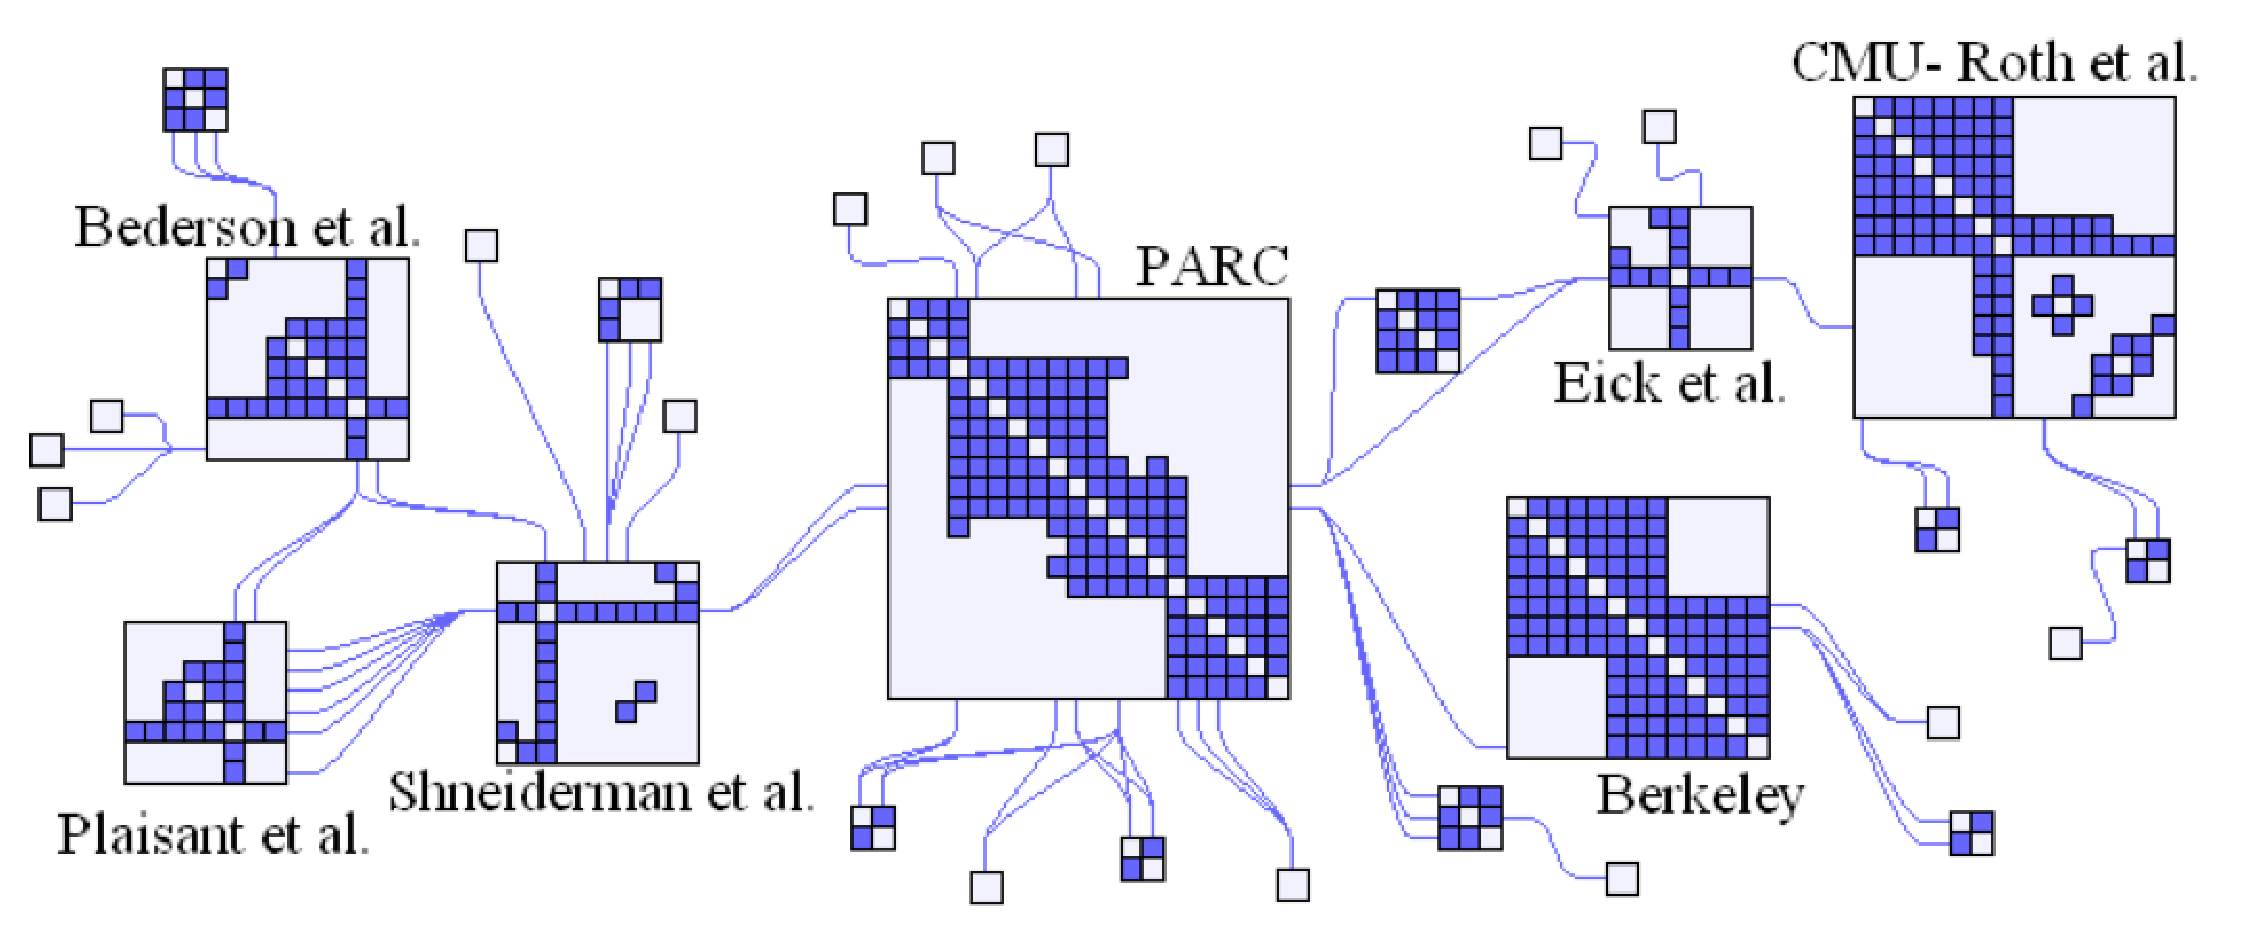
\includegraphics[width = 400px]{figures/nodetrix.eps}
  \caption{NodeTrix Representation of the largest component of the InfoVis Co-authorship Network ~\cite{henry2007nodetrix}}
  \label{fig:nodetrix}
\end{figure}

\textit{Semantic visualization}

Instead of highlighting the explicit relationships found in the data,
the semantic visualization focuses on representing the high level
attributes and connections of the nodes either as specified
explicitly in the data, or implicitly inferred from cross-referencing
externa sources.

Shen et al. proposed a visualization called OntoVis~\cite{shen2006visual} based on the
node-link method with a high-level graphical representation of the
ontology (See Figure \ref{fig:ontovis}).

\begin{figure}[!htb]
  \centering
  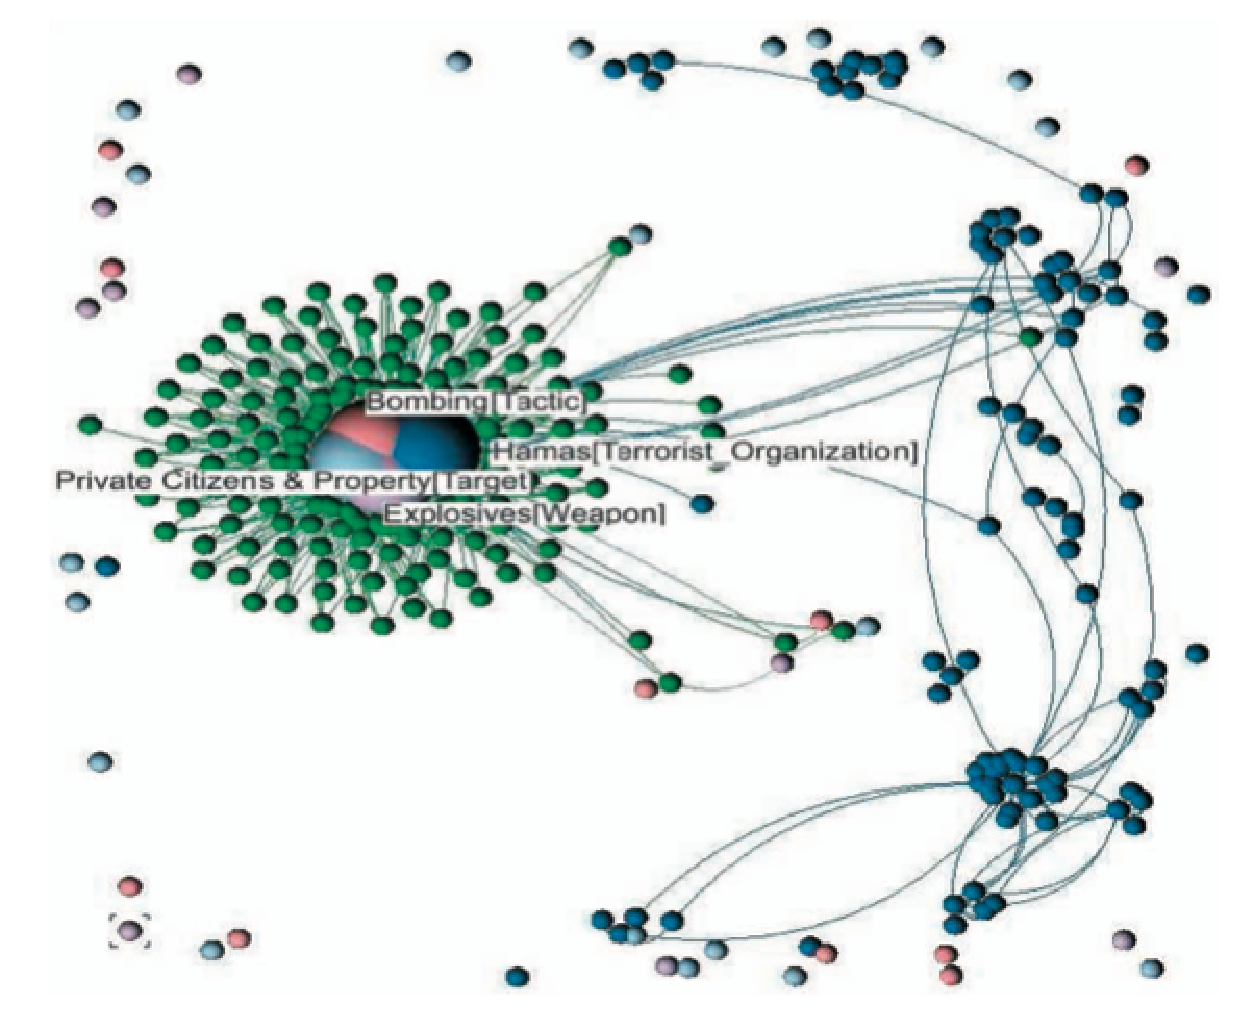
\includegraphics[width = 400px]{figures/ontovis.eps}
  \caption{Visualization of Terrorist Attacks (in green) Related to Hamas in 2005. Bombing is also the major tactic used by Hamas. However, their attacks focus on private citizens and properties. ~\cite{shen2006visual}}
  \label{fig:ontovis}
\end{figure}

\textit{Temporal visualization}:

The temporal information actually is a special type of high level
atrributes of the nodes or the edges in the graph. Since the social
interaction is a time-dependent phenomenon, it is only natural to
represent the temporal dimension visually. One of the
difficulties to represent time is a shortage of dimensions to depict a
dynamic network in a 2D display. As an alternative, one can represent
time along precisely one temporal demension. 

\textit{statistical visualization}:

The analysts are often interested in some statistical information,
which helps them to have an overview of the whole data and explore what
they need. This is at the core of visual analytics. The variables
often correspond to network statistics that represent the structure of
the network, such as degree, centrality~\cite{freeman1979centrality} and the clustering
coefficient. The first two describe the importance across the network,
the latter metric indicates how clusterable the nodes are in the social
network. 

\begin{figure}[!htb]
  \centering
  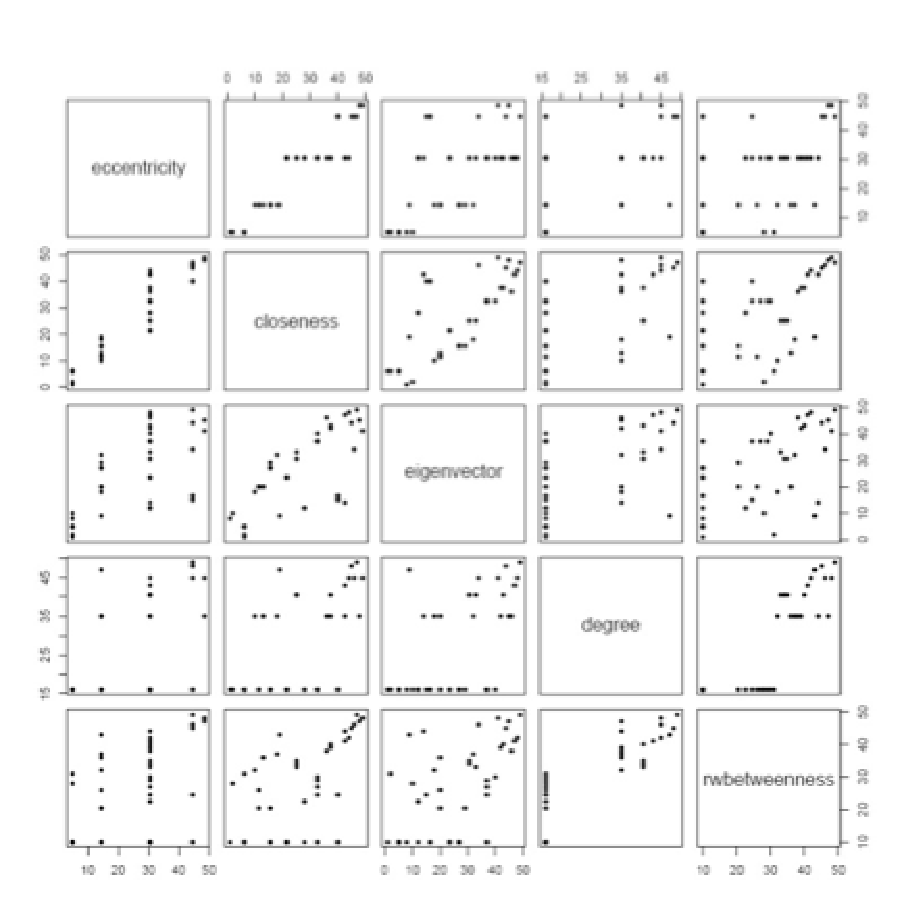
\includegraphics[width = 300px]{figures/plotmatrix.eps}
  \caption{An example of node-link method for the structure visualization ~\cite{dwyer2006visual}}
  \label{fig:plotmatrix}
\end{figure}

\begin{figure}[!htb]
  \centering
  \includegraphics[width = 350px]{figures/3dpc.eps}
  \caption{3D parallel coordinates for Padgett’s Florentine families marital relation data ~\cite{dwyer2006visual}}
  \label{fig:dpc}
\end{figure}


In general, network statistics form an N-dimensional space, where a
node or an edge is an observation, and each variable corresponds to an
attribute or metric. Dwyer et al. used a scatter plot matrix of common
centrality to understand the distribution of importance in social
networks~\cite{dwyer2006visual}, which is first used in
~\cite{koschutzki4comparison}. Dwyer et al. also used the 3D parallel
coordinates to represent the pairwise joint-distributions, which is to
represent each data point as a set of line segments whose endpoints
are the values of each of the variables (See Figure~\ref{fig:dpc}). Also, the scatter plots can
be used in representing the edge correlations. In
~\cite{goh2003betweenness}, Kahng et al. used this technique to study the
betweenness centrality correlation in social networks.

\section{Diffusion visualization}

\begin{figure}[!htb]
  \centering
  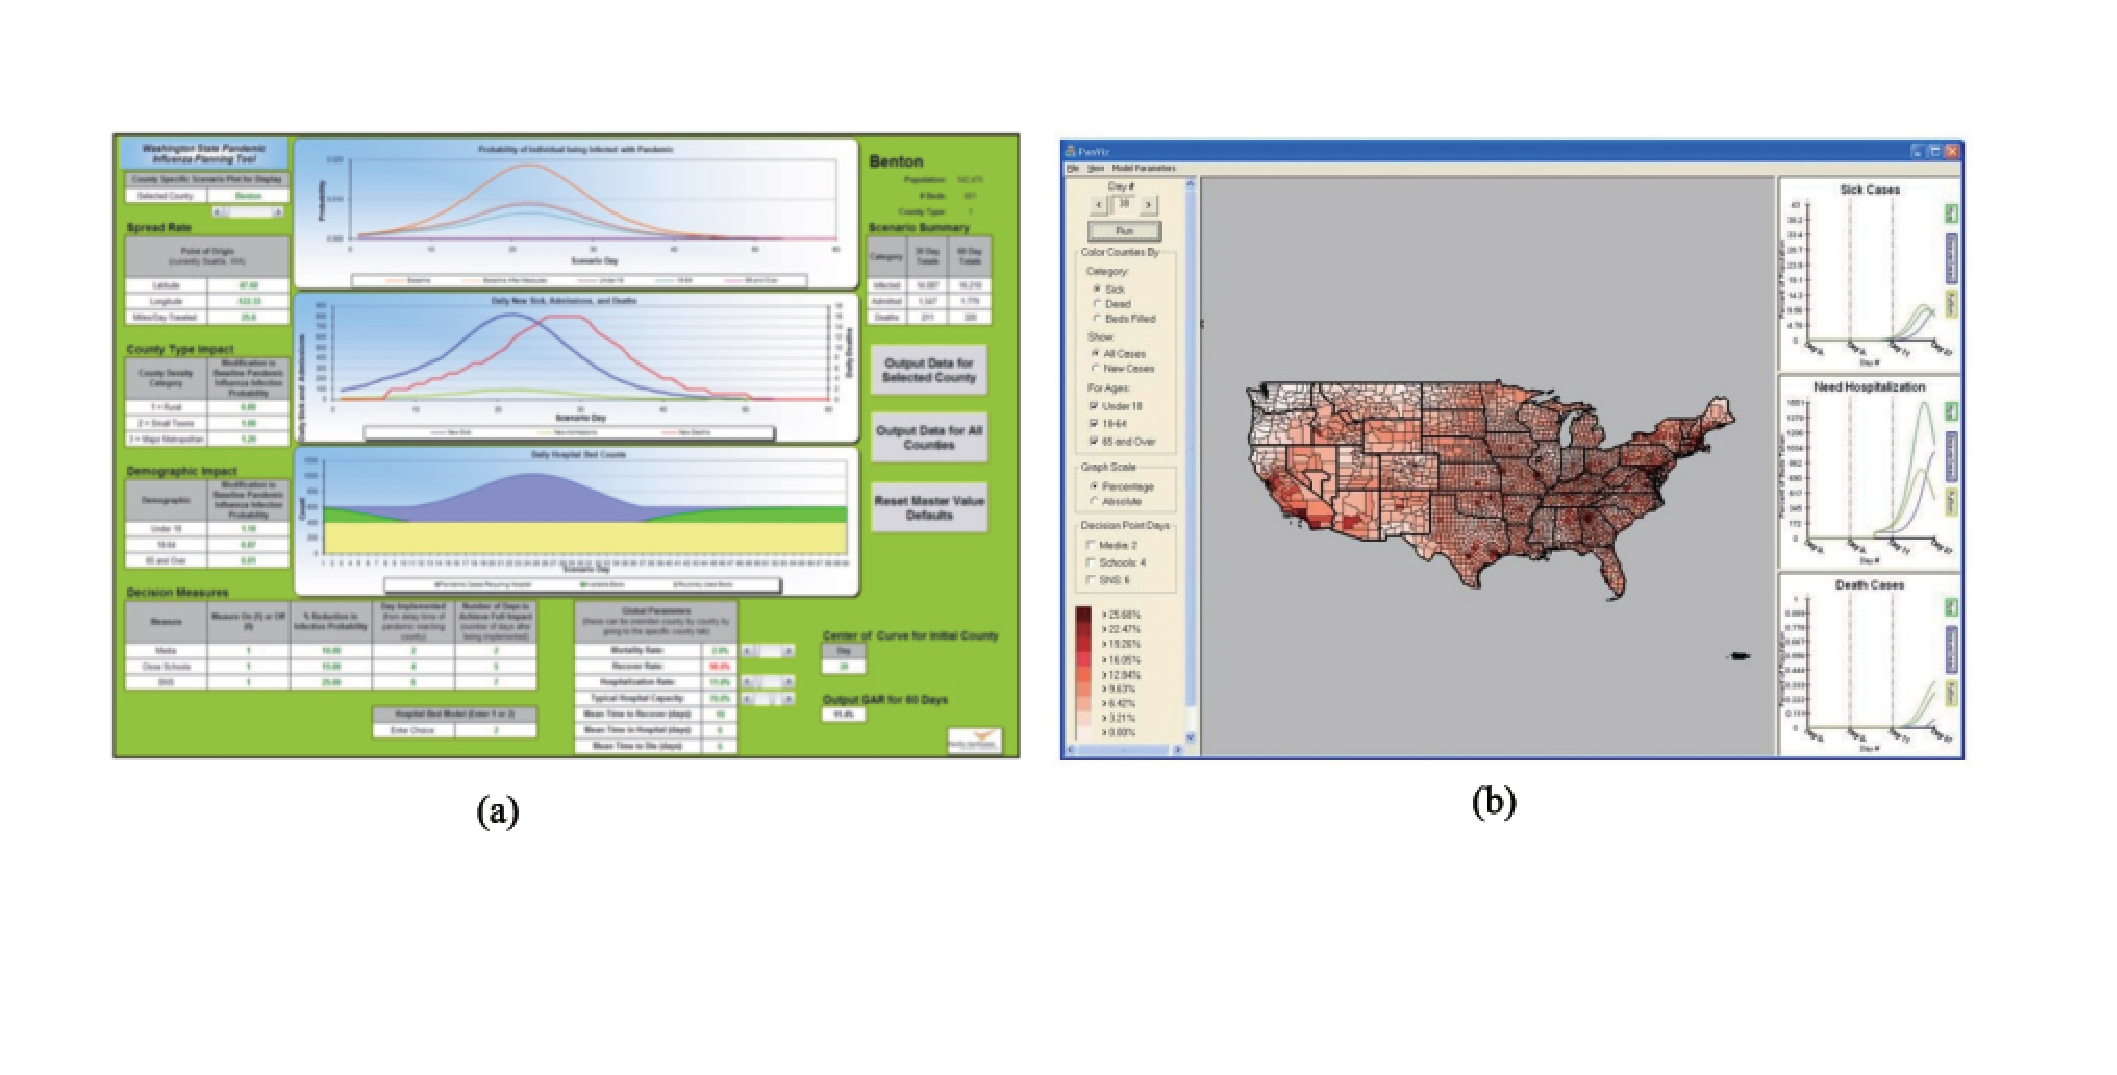
\includegraphics[width = 500]{figures/flu.eps}
  \caption{The Figure (a) shows the Pandemic Influenza Quick Look Tool
    Screenshot and Figure (b) shows the PanViz Applied at a National Level~\cite{brigantic2010development}}
  \label{fig:flu}
\end{figure}


To our best of knowledge, there is a lack of work on visualizing the
information diffusion for social networks. Nevertheless, Brigantic et
al. developed quick look tools (QLTs)  that can help the expert to clearly
see the Pandemic Influenza
modeling~\cite{brigantic2010development}. They claimed that, if an event 
happened, the QLTs could then be employed to rapidly assess and execute alternative mitigation strategies, and 
thereby minimize casualties.
 
\section{Other visualization techniques}

\begin{itemize}
\item Flow visualization

The information diffusion is just like the information flowing on the network. Thus, some techniques on flow visualization could be used. Flow visualization is a very big topic in scientific visualization
area and has being studied for many years. The flow visualization is about how to make flow pattern visible. In Figure. \ref{fig:flowvis} is an example.

\item Flow map
\begin{figure}[!htb]
  \centering
  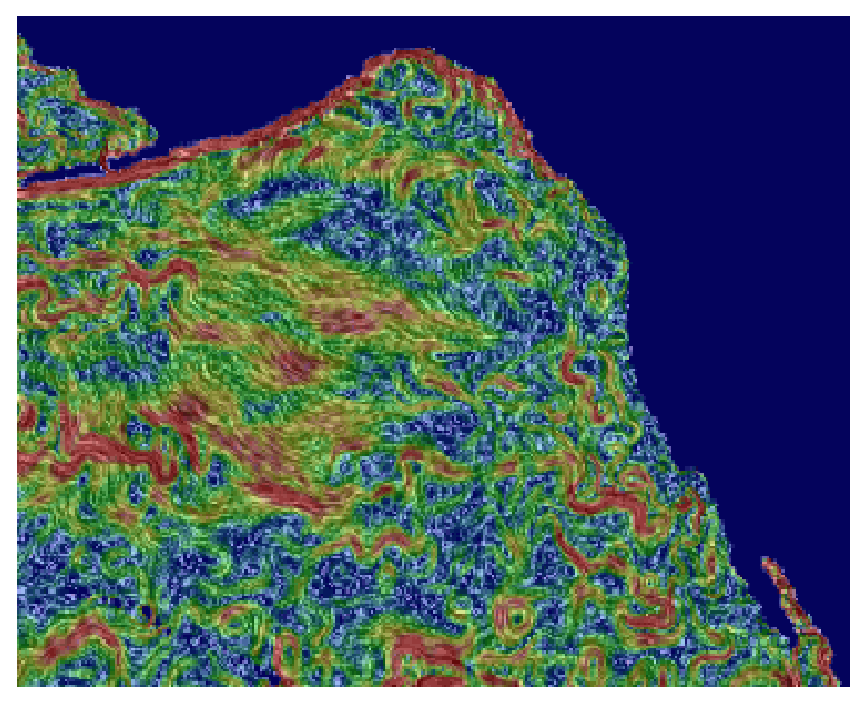
\includegraphics[width = 300]{figures/flowvis.eps}
  \caption{Flow visualization of the ocean current in the Northeast Pacific using the Line Interval Convolution technique. Red indicates areas of high magnitude flowand blue indicates areas of low magnitude flow.~\cite{moorhead1995signal}}
  \label{fig:flowvis}
\end{figure}

The flow map is a visualization to visualize the network flow and the topology and shows the spatial distribution of univariate geographic phenomena. Generally, in a flow map, the width of the lines will represent the size of the flow, and we can merge edegs sharing the destinations in order to reduce the clutter. In ~\cite{phan2005flow}, Phan proposed a method that can generate the flow map automatically (See Figure ~\ref{fig:flowmap}c).

\begin{figure}[!htb]
  \centering
  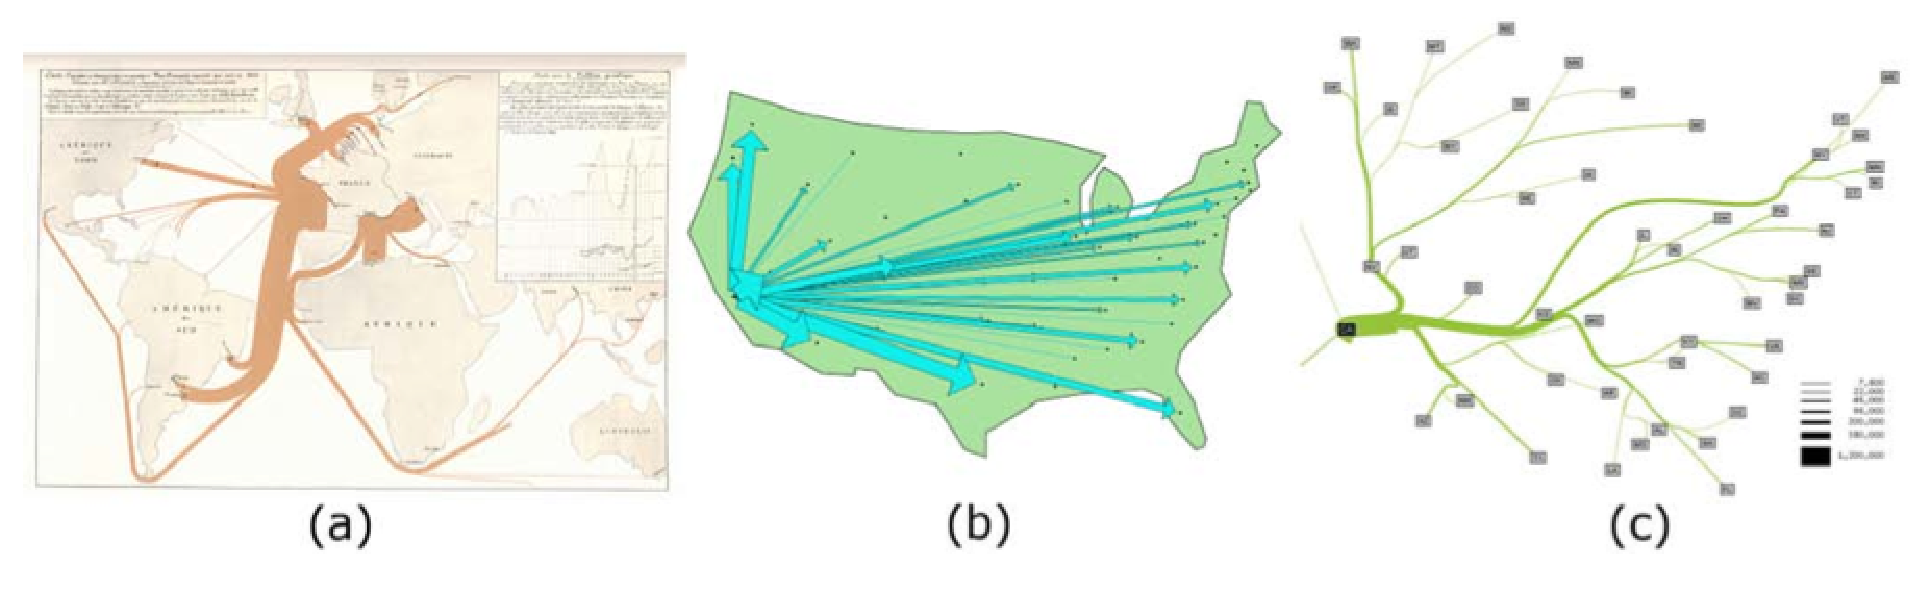
\includegraphics[width = 500]{figures/flowmap.eps}
  \caption{Flow maps. (a) Minard’s 1864 flow map of wine exports from France. (b) Tobler’s computer generated flow map of migration from California from 1995 - 2000. (c) A flow map produced by our system that shows the same migration data.~\cite{phan2005flow}}
  \label{fig:flowmap}
\end{figure}

\item Trajectory visualization
\begin{figure}[!htb]
  \centering
  \includegraphics[width = 270]{figures/tra.eps}
  \caption{The visualization to show the aircrafts' traffic over France in one day. The color represents the altitude of the aircraft: the green represents the lowest altitude and the blue represents the highest altitude~\cite{hurter2009fromdady}.}
  \label{fig:tra}
\end{figure}

\begin{figure}[!htb]
  \centering
  \includegraphics[width = 300]{figures/tra2.eps}
  \caption{The visualization to show the density of the Dutch coast.\cite{willems2009visualization}}
  \label{fig:tra2}
\end{figure}

Trajectory visualization is trying to visualize the objects' movement based on their geographic information. There are several similarities between the diffusion visualization and trajectory visualization: 1) the data of the diffusion and the trajectory in temporal and spatial; 2) both the diffusion and the trajectory are based on the graphs. One of the major differences is that for the trajectory data, the geographic position is a key information to visualize. However, for the data of information diffusion on soical media, in most situation, there will be no geographic information. Thus, if we want to use the technology for the trajectory visualization, this is the importance issue that we should consider. Figure~\ref{fig:tra} and Figure~\ref{fig:tra2} are the examples for the trajectory visualization.

\end{itemize}
